%!TEX root = ../dissertation.tex
\chapter{Demonstration of Technology}
\label{chap:demonstration}
This section will demonstrate a few applications of the framework presented in this thesis. Applications include simulations of articular cartilage during the gait cycle, fluid-solid interaction in complaint robotics, and continuum granular flow simulation.

\section{Simulation of Articular Cartilage}\label{sec:AC_model}
Tibiofemoral articular cartilage withstands compressive loads of multiple times body weight during walking, and transmits forces across skeletal joints while distributing the loading on the underlying subchondral bone \cite{Kutzner2010}. This mechanical purpose factors into cartilage health, as normal tissue function requires homeostasis, a balance of tissue remodeling and degradation regulated in part by the repetitive loading experienced during functional movements \cite{griffin2005}.

The substantial load-bearing capacity of this multiphase tissue is provided by the extracellular matrix, a multiphase tissue composed of an ionized fluid and a solid network of collagen fibers and embedded macromolecules. The electrostatic attraction between proteoglycan macromolecules and the ionic fluid leads to an osmotic pressurization of the extracellular matrix. This internal pressure is equilibrated by tensile loading in the collagen fibers. When cartilage is loaded, the contact loads are distributed throughout the tissue via further pressurization of the interstitial fluid \cite{Cohen1998, Fox2009}. This combination of interstitial fluid pressure and compressive and shearing contact loads results in a complex loading environment for the collagen fibers \cite{Briant2015,Kaab1998,Notzli1997}. Characterization of this collagen fiber loading during functional movement is critical to understand the superficial cartilage degradation and fibrillation associated with the initiation of osteoarthritis \cite{Andriacchi2004,Carter2004,griffin2005,Poole2002}.

Collagen fibers exhibit distinct patterns in orientation throughout the cartilage tissue. In the depth-wise direction, fibers extend vertically from the subchondral bone, bend through the mid-layer and lie parallel to the articular surface in the superficial layer \cite{Benninghoff1925}. Within the superficial layer, the fibers exhibit preferential orientation along the articular surface as well. This superficial collagen fiber orientation is revealed through split lines produced by inserting a needle coated in India ink into the tissue \cite{Below2002,Benninghoff1925,Responte2007}.Collagen fiber orientation produces significant anisotropy in the tissue mechanical properties, demonstrated by increased tensile stiffness along the split line direction \cite{Sasazaki2006}.  Although the physiologic mechanism linking collagen alignment to loading is still uncertain, an enzyme that selectively degrades unloaded collagen fibers may provide this link \cite{Nabeshima1996,Ruberti2005}. At the tissue level, the link between loading and collagen orientation remains difficult to study, because while Magnetic Resonance Imaging (MRI) based techniques to quantify tissue strains have recently been introduced, they are limited in their ability to study functional movement \cite{Lad2016,Chan2016}.

To overcome the limitations of current experimental techniques, computer simulation is often used to investigate cartilage loading. To properly model the loading scenarios that contribute to fiber orientation and the development of OA, simulations must resolve the net joint loading during locomotor movements and the corresponding internal joint tissue stresses. Simultaneous solution for the muscle forces that produce a movement and detailed internal joint mechanics results in intractable computational complexity. As a result, a muscle driven multibody simulation with a simplified knee model is often performed first to determine the net joint loads, which are then used as inputs to a detailed finite element model to solve for internal cartilage tissue stresses \cite{Halloran2012,besier2005modeling,klodowski2016merge}. Finite element models of cartilage of increasing complexity have been introduced including linear elastic, multiphase, and fibril reinforced to accurately capture the response of cartilage to applied loads \cite{Halloran2012,klika2016overview,Julkunen2013}. Recently, simulation routines have been introduced that model cartilage contact using an elastic foundation representations to allow for internal joint mechanics to be solved simultaneously with the musculoskeletal dynamics \cite{Smith2016influence2,Lenhart2015,Marra2015,Guess2013}. However, these improved musculoskeletal simulation techniques have not been extended to resolve internal tissue stresses.

The aforementioned simulation techniques have been used previously to gain insight into the connection between cartilage loading and collagen orientation. Experimentally measured cartilage split line orientations have been included in fiber-reinforced finite element models to study their influence on predicted cartilage strain patterns \cite{Shim2016,Mononen2012,Li2016}. Other researchers have developed remodeling laws based on mechanical parameters such as the directions of principal strains to predict collagen alignment \cite{Wilson2006,Cortez2016}. However, these works are limited to simplified geometries and loading conditions and have only been applied to depth-wise collagen orientation. Thus, it remains unknown whether cartilage split line directions correspond to mechanical loading during locomotion.

In the preset work, a novel simulation framework which integrates kinematic and kinetic measurements of full body movement with a muscle-driven image based model of the knee joint to predict superficial cartilage layer mechanics was investigated. The model and simulation framework is then used to predict cartilage surface strains due to passive osmotic pressure and a simulated walking cycle. The orientation of the principal strains in the cartilage surface are compared against experimentally measured split lines to provide insight into the connection between fiber loading and orientation.

\subsection{Computational model}
\label{ss:ComputationalAC}

This section outlines the basic ideas behind the computer implementations used to model the geometry and deformation of the AC surfaces and their contact.

A three-body, 12 degree-of-freedom (DOF) knee model was developed from magnetic resonance (MR) images of a healthy adult female (1.65\, m, 61\,kg). Details of model development have been previously published \cite{Lenhart2015}, but will be briefly summarized for clarity. Fourteen ligaments were represented by bundles of nonlinear elastic springs, with wrapping surfaces included to prevent penetration of bony geometries. Articular cartilage surfaces were segmented from the MR images and represented by high-resolution meshes. Cartilage contact pressures were calculated based on the overlap depth between the articulating surfaces using an elastic foundation model. The knee model was integrated into an existing lower extremity musculoskeletal model \cite{Arnold2010}, which included 43 muscles acting about the hip, knee and ankle joints. The predictive capacity of the model was validated by comparing simulated passive and active knee kinematics with in vivo 3D knee kinematics measured with dynamic MRI \cite{Lenhart2015}.

Tibio-femoral kinematics during walking were predicted using the Concurrent Optimization of Muscle Activations and Kinematics (COMAK) simulation routine \cite{Smith2016,Smith2016influence2}. Whole-body kinematics and ground reactions were recorded while the subject walked overground in a motion analysis laboratory. At each frame of a gait cycle, numerical optimization was used to calculate the muscle forces, patello-femoral kinematics and secondary tibio-femoral kinematics that minimized a weighted sum of squared muscle activations cost function while satisfying overall dynamic constraints. The constraints required that the muscle forces and internal knee loads (contact pressures, ligament forces) produced by the optimized knee kinematics generate the measured hip, knee (flexion) and ankle accelerations. In the present study, the six degree-of-freedom patello-femoral kinematics is used to drive the motion.


The AC surface is modeled with shell finite elements using the ANCF method described in \S\ref{sec:2DElem}. Handling of contact represents a key computational challenge for the accurate simulation of deformable meshes. The deformable AC surface model presented in this thesis relies on the triangularization of quad meshes, where each quad (shell) is split into two triangles, thereby defining vertices, faces, and edges. By making use of broad and narrow phases, the shell element meshes are checked for contact by evaluating interpenetrations between vertices and faces, and between edges and edges. If contact is likely to occur, geometrical information, such as the location of the contact point, normal direction, interpenetration, and interpenetration velocity are calculated for each vertex-face and edge-edge pair. A penalty formulation is used to generate normal forces; to ensure the desired accuracy, contact stiffness parameters and time steps are selected such that the maximum mesh interpenetration is from one to two orders of magnitude smaller than the actual deflection of AC surfaces. Fig.~\ref{fig:contact} depicts a scheme of the triangularization of the finite element meshes and the geometric entities that intervene in contact detection.
\begin{figure}[H]
	\begin{center}
		\includegraphics[width=0.50\columnwidth]{images/AC/contact.png}
		\caption{Triangular mesh for AC surface vs surface contact. The quad finite element mesh is first converted to a triangular mesh composed of vertices, edges, and faces. Each vertex is associated with a normal vector to compute interpenetrations. }\label{fig:contact}
	\end{center}
\end{figure}
The overview of the current case study is illustrated in Fig.~\ref{fig:overview}.
\begin{figure}[H]
	\begin{center}
		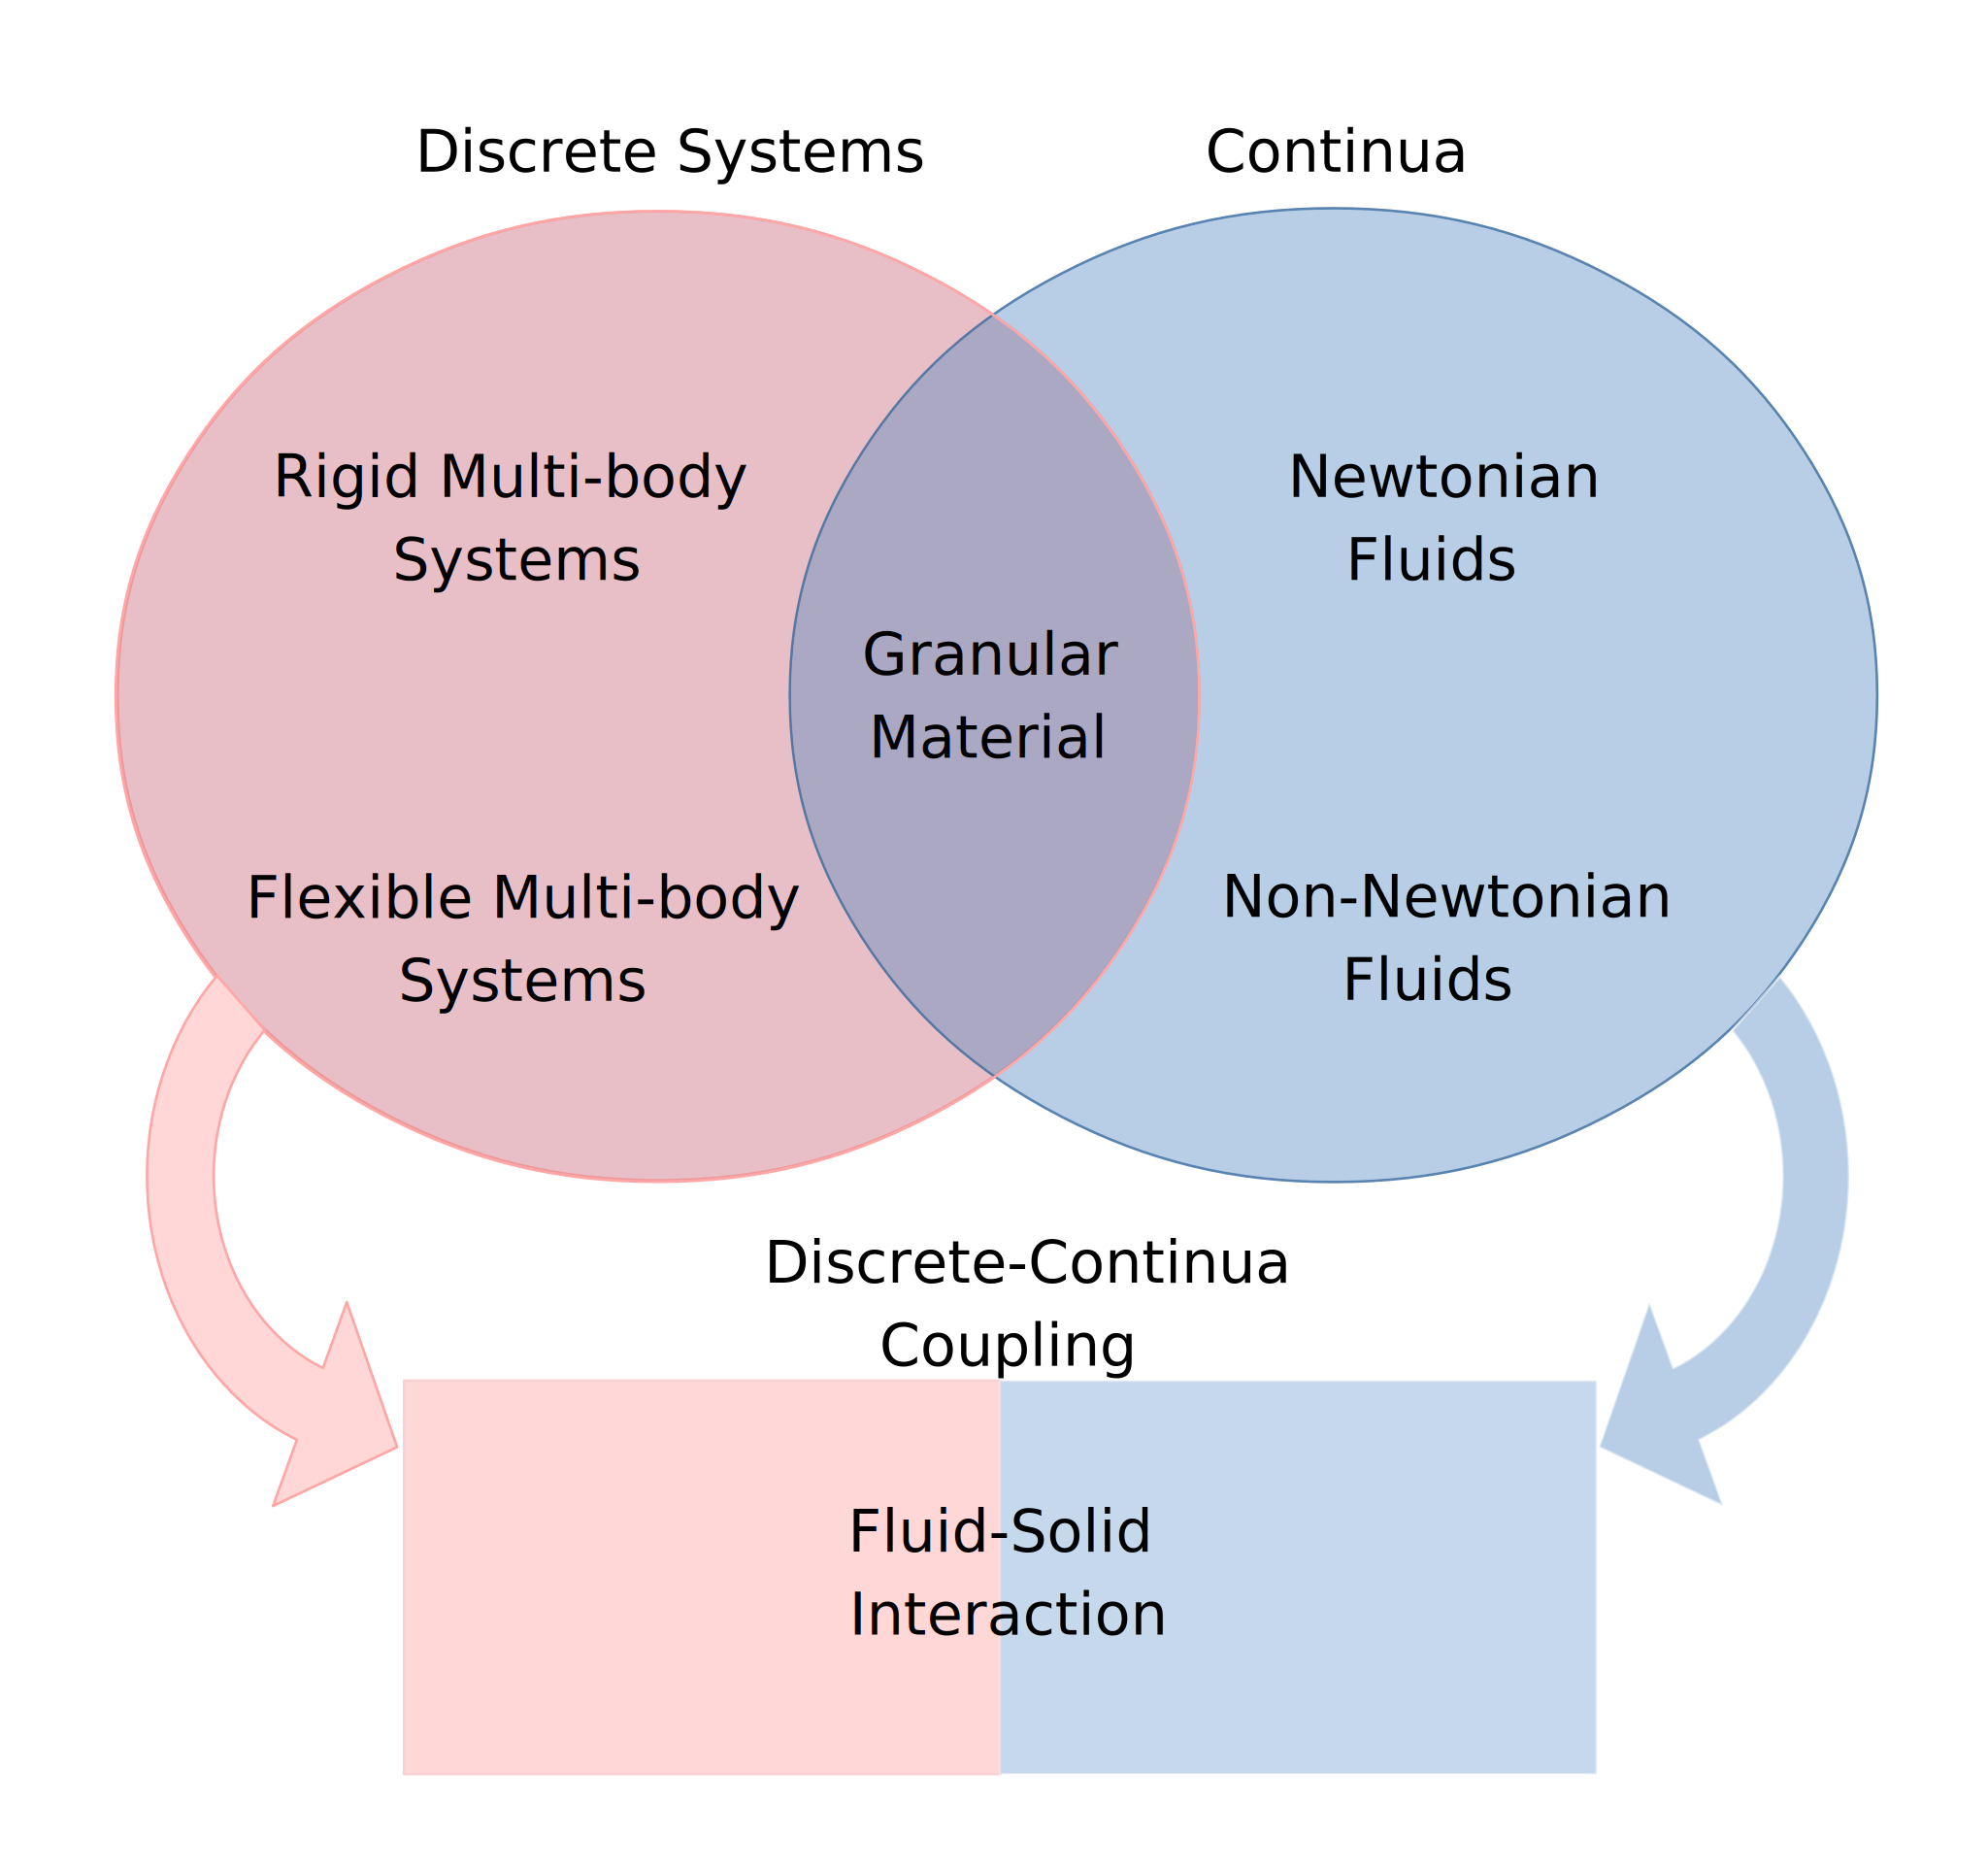
\includegraphics[width=0.98\columnwidth]{images/AC/Overview.pdf}
		\caption{Overview of the two-step simulation process. First, a musculoskeletal dynamic simulation (COMAK), including an elastic foundation contact model, was used to solve for tibiofemoral knee kinematics. Then, a novel deformable model was used to estimate superficial cartilage strain at each instant in the gait cycle. Finally, the average first principal strain directions were visually compared with experimental split line maps (\cite{Below2002}) which represent collagen fiber alignment.}
		\label{fig:overview}
	\end{center}
\end{figure}

\subsection{Results}
\label{sec:Results}
The model is verified by comparing $i)$ tibio-femoral contact forces and $ii)$ deflection of the femur and tibia cartilages obtained from the deformable-surface model against those predicted by the rigid-surface model~(\cite{Smith2016}). The schematic comparison of the two methods is illustrated in Fig.~\ref{fig:comparison}.

\begin{figure}
	\begin{center}
		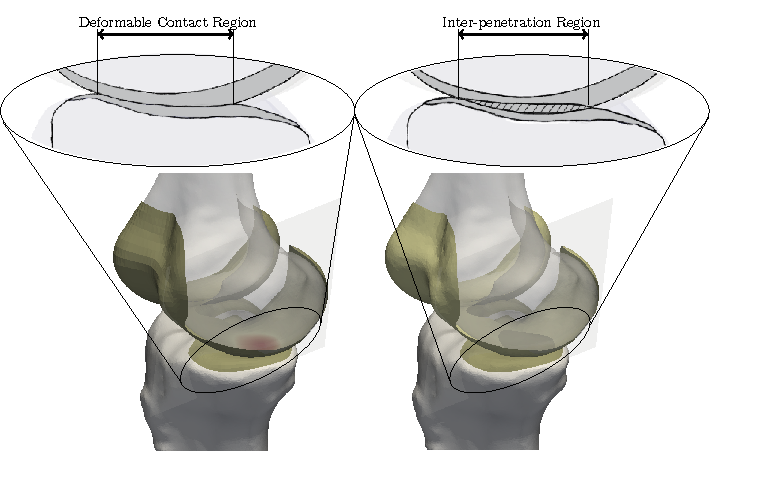
\includegraphics[width=0.8\columnwidth]{images/AC/Comparison.png}
		\caption{Schematic comparison of the elastic foundation model (left) with the deformable model (right) with the 2D section views on top.}\label{fig:comparison}
	\end{center}
\end{figure}

Tibio-femoral contact force patterns exhibit a characteristic double peak during stance, with the majority of the force passing through the medial compartment. Fig.~\ref{fig:netLoad} illustrates the comparison of the tibio-femoral contact forces predicted by the models. The time-averaged relative difference, $\overline{\frac{|x-x_{ref}|}{|x_{ref}|}}$, between the results of the present study and what has been reported in~(\cite{Smith2016}) for the net force in the superior-inferior direction, are $\approx 19\%$, $27\%$, for respectively medial and lateral compartments of tibia plateau and $ 17\%$ for the femur condyle. Considering the fundamental differences between the two models, the results of the present model are in good agreement with the established approach \cite{Smith2016} and is able to exhibit the characteristic double peak during stance.
\begin{figure}
	\begin{center}
		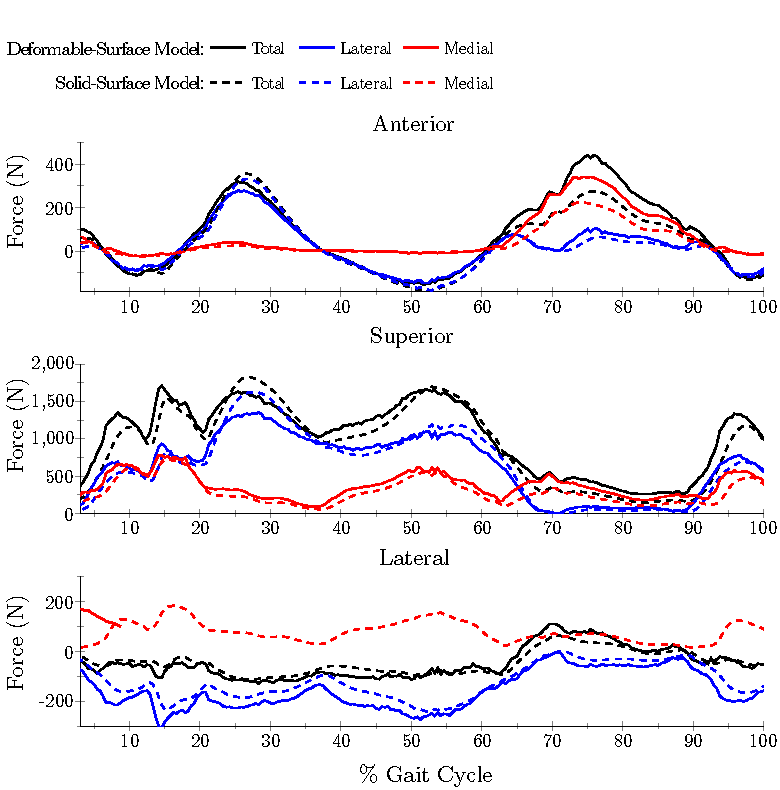
\includegraphics[width=0.7\columnwidth]{images/AC/NetLoad.png}
		\caption{Comparison of the net load results on the femur, medial and lateral cartilages with theelastic foundation model \cite{Smith2016}.}\label{fig:netLoad}
	\end{center}
\end{figure}
Fig.~\ref{fig:deflection} compares the deflected area of the femoral cartilage at the first peak of loading during the gait cycle between the two models. The deflection of each condyle in the solid-surface model is calculated based on half of the inter-penetration. As seen, the deflection in the deformable-surface model is more evenly distributed in the deflected area in comparison with the solid-surface model. In addition, regions away from the contact patch are more influenced by the deformable-surface model in comparison with the solid-surface model. Relative difference in maximum deflection is less than $1\%$ between the two model. Overall, the deflection field over the gait cycle shows acceptable agreement between the two models.\\
\begin{figure}[ht!]
	\centering
	\begin{subfigure}{0.48\columnwidth}
		\centering \hskip -5mm
		\includegraphics[height=0.65\textwidth]{images/AC/Comp-Sol.png}
		\caption*{\hspace{-0.5cm}Elastic foundation model \\ \hspace{-0.5cm}(\cite{Smith2016})}
	\end{subfigure}
	\begin{subfigure}{0.48\columnwidth}
		\centering
		\includegraphics[height=0.65\textwidth]{images/AC/Comp-Def.png}
		\caption*{\hspace{-2cm} Deformable model }
	\end{subfigure}	
	\caption{Comparison of articular cartilage inter-penetration (elastic foundation model) and deflection (deformable model). Also see Fig.~\ref{fig:comparison}}\label{fig:deflection}
	\end{figure}
\subsection*{Prediction of collagen fiber orientations}
The effects of two types of loading on the cartilage are investigated here: $(i)$ internal loading due to the cartilage internal pressure, and $(ii)$ external loading due to the gait cycle. The internal pressure of the cartilage is a function of the external load; as the compressive load on the cartilage increases, the fluid content of the cartilage is reduced and the internal pressure increases. Therefore, both effects should be investigated when studying the effect of loading on strain distribution/directions. Moreover, considering that tibio-femoral joint predominantly operates under the gait cycle during one's life, it can be  assumed that the gait cycle loading and the internal pressure determine the collagen fibers' direction. Many researchers have correlated the maximum principal strain direction to the collagen fiber orientation (e.g. see \cite{Below2002}). Hence, the deformable-surface model is used to obtain the principal strain directions for the aforementioned scenarios.

In the first scenario, the kinematics of the gait cycle loads the cartilage and no pressure is present. Fig.~\ref{fig:Femur_Gait} shows the principal strain direction vectors scaled by the magnitude of the principal strains at three representative instants of time during the gait cycle: Heal strike, first peak, and second peak. During the gait cycle, the largest first principal strains, $\epsilon_1$, are observed at the periphery of the cartilages, whereas, the most negative second principal strains, $\epsilon_2$, are observed at the regions where the femoral cartilage undergoes larger deflection, i.e. the central region. Due to the shape of the femoral cartilage at the medial side, the cartilage surface undergoes compressive loading at the center of the contact region as the principal strain of largest magnitude tends to be negative (Fig.~\ref{fig:Femur_Gait} first peak).
\begin{figure}
	\begin{center}
		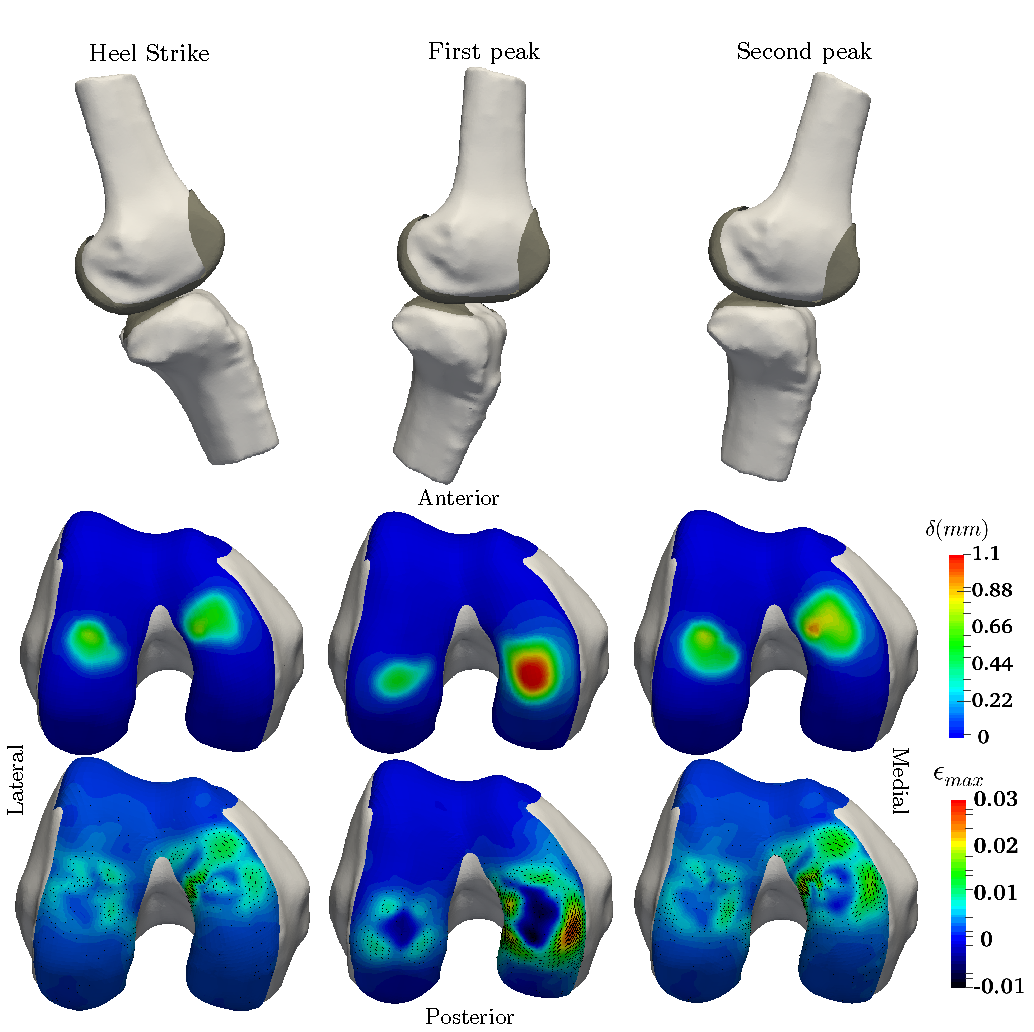
\includegraphics[width=\columnwidth]{images/AC/Femur_Gait.png}
		\caption{Different instants of time during the gait cycle when no internal pressure is applied. First row: schematic of the motion during the gait cycle. Second row: deflection field. Third row: maximum principal strains. Black lines show the first principal strain directions and are scaled by the magnitude of the first principal strain at each FE node. See Fig.~\ref{fig:Tibia} in supplementary information for corresponding tibial plateau pressures and strain patterns.}\label{fig:Femur_Gait}
	\end{center}
\end{figure}
In order to obtain a representative measure of principal strains over the gait cycle, the weighted principal strain directions are averaged over time. Fig.~\ref{fig:Femur}$(a)$ shows the split-line pattern obtained for this case. It may be observed that the maximum (first) principal strain directions due to external loading shows little similarities with the experimental results.

In the second scenario, only internal pressure is present. The magnitude of the applied pressure is $0.2$\,MPa which is the typical hydrostatic internal pressure of the cartilage. Fig.~\ref{fig:Femur}$(b)$ illustrates the maximum (first) principal strain direction for this case. Comparison of the maximum principal strain directions with experimental split-line patterns shows very good agreement.

\begin{figure}[H]
	\begin{center}
		\includegraphics[width=\columnwidth]{images/AC/Femur-Revised.png}
		\caption{Comparison of the fiber alignment predicted by this study for different scenarios with experimental results \cite{Below2002} on the femur condyle. Histograms demonstrate the distribution of the angle of deviation between the experimental split lines and predicted principal strain directions. The dashed lines on histograms show the median angle of deviation. See Fig.~\ref{fig:Tibia} in supplementary information for simulated first principal strain directions on the tibial plateau.}\label{fig:Femur}
	\end{center}
\end{figure}

\begin{figure}[H]
	\begin{center}
		\includegraphics[width=\columnwidth]{images/AC/Tibia_Gait.png}
		\caption{Different instants of time during the gait cycle when no internal pressure is applied. First row: schematic of the motion during the gait cycle. Second row: deflection field. Third row: maximum principal strains (black lines show the maximum principal strain directions and are scaled by the magnitude of the principal strain at each FE node.}\label{fig:Tibia_Gait}
	\end{center}
\end{figure}

\begin{figure}[H]
	\begin{center}
		\includegraphics[width=\columnwidth]{images/AC/Tibia-Revised.pdf}
		\caption{Comparison of the average first principal strain directions induced via (a) tibiofemoral loading during gait, (b) internal pressure and (c) coupled gait loading and  internal pressure.}\label{fig:Tibia}
	\end{center}
\end{figure}

Finally, both scenarios can be combined in one simulation in order to see whether one of them dominates the other or both scenarios equally affect the split-line pattern (see Fig.~\ref{fig:Femur}$(c)$). The comparison between Fig.~\ref{fig:Femur}$(a)$ and Fig.~\ref{fig:Femur}$(c)$ shows that, for the selected internal pressure level, the maximum principal strain is dominated by the gait cycle simulation. The lower the internal pressure, the smaller the resulting principal strains and the smaller contribution to the total split-line pattern. Conversely, with the application of larger internal pressures, the magnitude of the principal strain becomes dominant; therefore, Fig.~\ref{fig:Femur}$(c)$ would become closer to Fig.~\ref{fig:Femur}$(b)$.\\


\subsection{Discussion}
\label{sec:AC-Discussion}
The methodology used in the present study differs from the rigid-surface approach, the prevalent method that is used to resolve the internal joint loads in AC along with the musculoskeletal dynamics \cite{Smith2016,Lenhart2015,Marra2015,Guess2013}. In the solid-surface model, the deformation for each element is independent of neighboring elements and is simply approximated according to inter-penetration of two solid surfaces representing articular surfaces. The solid-surface model has been shown \cite{Guess2013,abraham2013} to be able to predict the contact pressure fairly well when compared to FE models, but it essentially does not resolve the internal tissue stresses. In contrast, the deformable-surface model captures the deformation of the articular surface and consequently allows for studying the tissue level stresses and mechanical behavior of the superficial region of the AC in more details. Therefore, properties such as strain directions, which are of interest in the current study, can be captured using this method. The higher-fidelity method, however, comes at a higher computational cost in comparison to the solid-surface model.

Moreover, the modeling technique used in the present work removes a number of the limitations of previous studies.  Previously, remodeling laws were used in an attempt to characterize the collagen fibers direction, but only simplified loading scenarios and simplified geometries \cite{Wilson2006} and depth-wise orientation of fibers \cite{Cortez2016} were investigated. In the present study, principal directions on AC surface were investigated for the actual geometry of the articular surface and during the gait motion. Overall, this study improves our understanding of how the collagen fibers orientation is directed by the mechanical conditions at the surface of the articular cartilage, which is of interest in areas such as tissue-engineering.

The results obtained from the current study suggest that depending on the type of the mechanical loading applied on articular surface, different predicted patterns for collagen fibers will emerge. Among these types of loading, the patterns we obtained due to the internal pressure more closely match the experimental results. This suggests that the surface-wise collagen fibers alignment might be tied to internal loads. Nonetheless, the external loadings such as gait motion can still indirectly affect the split-line patterns by increasing the internal pressure of the articular cartilage. See \cite{rakhsha2019simulation} for more details about this model.

\section{Continuum Simulation of Granular Flows}

In large, rigid multibody dynamics problems with friction and contact, encountered for instance in granular flows, one can witness distinctly different system-level dynamics. This section concentrates on the case of fluid-like behavior of large multibody dynamics systems such as granular materials, when the system experiences large strains. The results reported herein draw the Newton-Euler equations discussed in section~\S\ref{sec:RigidBody} for capturing the dynamics of granular flows in a discrete sense. In the continuum sense, the modeling approach discussed in in sections \S\ref{sec:Newtonian}-\S\ref{sec:granular_material} is employed. To demonstrate the similarities and differences between the multibody and fluid dynamics we consider three problems modeled and solved using different methods; ($i$) a compressibility test; ($ii$) the classical dam break problem, and ($iii$) the dam break simulation with an obstacle. These experiments provide insights into conditions under which one can expect similar characteristics from multibody and fluid dynamics systems governed by manifestly different equations of motion and solved by vastly different numerical solution methods. 

Herein, dynamics of spheres of identical radii is captured via the Discrete Element Method (DEM). In this approach, the time evolution of the rigid sphere $i$ is expressed as
\begin{subequations}
	\begin{equation}
	\label{eq:momentum_cons}	
	m \frac{d{\bf v}_i}{dt} = m {\bf f}_i + \sum_{i \neq j} \left({\bf F}_n^{ij} + {\bf F}_t^{ij} \right) \; ,
	\end{equation}
	where 
	\begin{align}
	\label{eq:FnFt}
	&{\bf F}_n^{ij} = f\left( \frac{\delta^{ij}}{2R} \right) \left( k_n \delta^{ij} {\bf n}^{ij} - \gamma_n \bar{m} {\bf v}_{n}^{ij} \right), \text{and} \\
	&{\bf F}_t^{ij} = f\left( \frac{\delta^{ij}}{2R} \right) \left( -k_t {\bf u}_t^{ij} - \gamma_t \bar{m}{\bf v}_t^{ij} \right),
	\end{align}
\end{subequations} 
are, respectively, the normal and tangential contact forces; $k_n$ and $k_t$ indicate stiffnesses; and $\gamma_n$ and $\gamma_t$  are damping coefficients for the normal and tangential directions, respectively. Above, $m$ is the mass of particles, $\bar{m}$ is an effective mass,  ${\bf v}_i$  is the velocity of particle $i$, $\delta^{ij}$ represents the mutual deformation of two elements in contact, and ${\bf f}_i$ represent an external force density such as gravity ($\bf g$). 

Once all contact forces and resultant accelerations are computed for timestep $k$, the latter are numerically integrated to yield the new velocity and position at timestep $k+1$. Different choices of time-integration methods \cite{hairer2009odeBook} such as Explicit Euler, Extended Taylor, and a second-order integrator proposed by Chung \cite{chungExplicit1994} are possible. The latter integrator assumes the form
\begin{equation}
\begin{aligned}
\label{eq:Chung}
{\bf v}_{k+1} &= {\bf v}_k + \Delta t \left( \frac{3}{2}{\bf a}_{k}  - \frac{1}{2}{\bf a}_{k - 1}\right)\\
{\bf x}_{k+1} &= {\bf x}_k + {\bf v}_k \Delta t + (\Delta t)^2 \left( \beta {\bf a}_{k} + \left( \frac{1}{2} - \beta \right) {\bf a}_{k-1} \right) \; .
\end{aligned}
\end{equation}	
It draws on a multistep approach, providing second-order integration for both position and velocity and strong numerical damping. On the down side, the Chung approach requires the caching of previous accelerations ${\bf a}_{k-1}$, increasing the memory overhead. It also provides $\beta$ as a tunable parameter for the integrator's numerical damping, with the stability requirement that $1 \leq \beta \leq \frac{28}{27}$. 

\subsection{Bucket of Material}
In this benchmark test we consider a bucket filled up with material -- in one case fluid, and granular material in a second case. We compare the magnitude of the average force on the side walls of the container for both media. This averaged force changes vertically. For the fluid media, there exists an analytical solution that comes from the hydrostatic fluid state. According to hydrostatic fluids, the pressure distribution is linear across the depth of the bucket -- the larger the depth, the higher the force impressed on the wall. Consequently, it is easy to show that the \textit{averaged} pressure (normal) force on each side of the container is $ \rho g h^2 L /2 $, where $h$ is the depth of the fluid in the bucket and $L$ is the length of side wall.  Furthermore, the ratio of this force to the weight of the material in the bucket for a $L$x$L$x$h$ fluid domain is $r_f=h/2L$. We performed DEM simulation to evaluate this ratio for a granular media instead of a fluid media. We calculate this ratio in granular material according to $r_g=\frac{\overline{|\textbf{F}_n|}}{Mg}$, where  $\overline{|\textbf{F}_n|}$ is the averaged normal forces across the side walls of the container, $M$ is the total mass of the system, and $g$ is the gravity. Finally, we calculate the relative error according to $e=\frac{r_f-r_g}{r_f}\times 100$. As shown in Fig.~\ref{fig:bucket}, the relative error is considerably small for the $h$ values that were simulated for a bucket of material with $L$= 1\si{m}.
\begin{figure}[H]
	\begin{center}
		\includegraphics[width=.8\textwidth]{images/CFD_DEM/Figure_Bucket.png}
	\end{center}
	\caption{The relative error of dimensionless normal force  experienced by the side walls of a bucket of material for different height ($h$) of material. The relative error is calculated according to $e=\frac{r_f-r_g}{r_f}\times 100$, where $r_f$ is the non-dimensional averaged fluid normal force and $r_g$ is the non-dimensional averaged granular normal force on the side walls. The $r_g$ is calculated from the DEM simulation while $r_f$ is computed from hydrostatic fluids.}
	\label{fig:bucket}
\end{figure}

We hypothesize that there should be a perfect agreement between the two media for this test and attribute the relative error seen in Fig.~\ref{fig:bucket} to mainly two factors: $(i)$ numerical errors of the DEM simulations; and $(ii)$ numerical errors associated with approximating the height of the granular material bucket from the particles' information. It is important to note that the DEM simulations were performed with \textit{frictionless monodisperse spherical} particles. We emphasize that $r_g$ is  different for frictional particles. A detailed discussion on the interplay between the friction forces and the side walls, as well as on the sensitivity of the results with respect to the particles' shape goes beyond the scope of this contribution and is the subject of ongoing work and goes beyond the scope of the current thesis.


\subsection{Material Column Collapse}
The initial domain of the material is 2\si{m}x4\si{m}x2\si{m}, while 6\si{m}x4\si{m}x4\si{m} is the size of the container. The reference density is $\rho=1000$ \si{kg/m^3}, and the gravity of $g=-9.8$ \si{m/s^2} is applied in the $y$ direction.

We study the propagating wave front both in granular material flow and the fluid flow. We highlight the similarities in terms of front speed as shown in Fig.~\ref{fig:front_pos}, and the differences in terms of the two characteristics of the dam break simulation, i.e. the \textit{roll up} and the \textit{second splash} \cite{miladHalfImplicit2018} as shown in Fig.~\ref{fig:dambreak}.
\begin{figure}[H]
	\begin{center}
		\includegraphics[width=.6\textwidth]{images/CFD_DEM/Figure_Dambreak.png}
	\end{center}
	\caption{Comparison of the front position in the dam break simulated with DEM and CFD.}
	\label{fig:front_pos}
\end{figure}
\begin{figure}[H]
	\centering
	\begin{subfigure}{0.45 \textwidth}	
		\centering
		\includegraphics[width=1.0\textwidth]{images/CFD_DEM/colorBar.png}
	\end{subfigure}
	
	\hspace{-0.2cm}
	\begin{subfigure}{0.45 \textwidth}	
		\centering
		\includegraphics[width=1.0\textwidth]{images/CFD_DEM/cfd_rollup.png}
	\end{subfigure}
	\begin{subfigure}{0.45 \textwidth}
		\centering
		\includegraphics[width=1.0\textwidth]{images/CFD_DEM/cfd_secondSplash.png}
	\end{subfigure}
	%
	\begin{subfigure}{0.45 \textwidth}	
		\centering
		\includegraphics[width=1.0\textwidth]{images/CFD_DEM/dem_rollup.png}
	\end{subfigure}
	\begin{subfigure}{0.45 \textwidth}
		\centering
		\includegraphics[width=1.0\textwidth]{images/CFD_DEM/dem_secondSplash.png}
	\end{subfigure}	
	\caption{Comparison of the roll up (left) and the second splash (right) instances of the dam break simulation between granular (bottom) and fluid (top) mediums.}	\label{fig:dambreak}
\end{figure} 
Considering that the CFD and the DEM solvers solved different governing equations, the similarity that is seen in terms of front propagation position is somewhat perplexing. However, as shown in Fig.~\ref{fig:front_pos}, the front position predicted by the DEM simulation moves slightly slower than the one predicted by the CFD solver. We attribute this discrepancy to the bulk density of the material; applying $\rho=1000$ \si{kg/m^3} to individual grains results in smaller overall density in granular material. This is true because of the nature of the packing in granular material, which allows for empty spaces between the grains. This feature, for example, guarantees that a bucket of sand is lighter than a bucket of fluid, assuming that the density of grains is equal to density of the fluid and the buckets have similar dimensions. Hence, we hypothesize that the slower front speed is due to lighter material in DEM simulation. On the CFD side only, a more ample discussion of this test may be found in \cite{Adami2012,miladHalfImplicit2018}.

\subsection{Column Collapse with an Obstacle}
In this experiment we placed a rigid cylindrical obstacle in front of the dam and monitor the overall force experienced by the cylinder over time after the dam breaks. The configuration of the problem is as follows: 2\si{m}x4\si{m}x2\si{m} is the initial domain of the material, and 6\si{m}x4\si{m}x4\si{m} is the size of the container. The dam is place in the leftmost corner of the domain and a 4 meter tall cylinder with the radius of 0.3\si{m} is placed at $x=5$\si{m} from the leftmost side of the container. Figure~\ref{fig:db_obstacle} demonstrates the force experienced by the cylinder for both the granular and the fluid material for different fluid's viscosities, and different grains diameter. As shown in Fig.~\ref{fig:db_obstacle}, within the simulated range, the viscous forces in the fluid simulation do not play a major role in the overall force on the cylinder. Similarly for granular flow, the force exerted on the cylinder is virtually insensitive to the particles' diameter. 

\begin{figure}[H]
	\begin{center}
		\includegraphics[width=.8\textwidth]{images/CFD_DEM/Figure_Dambreak_obstacle.png}
	\end{center}
	\caption{Comparison of the normalized horizontal force experienced by the cylinder in the dam break simulation for different viscosities of the fluid and for different particle diameters of the granular media.}
	\label{fig:db_obstacle}
\end{figure}

Assuming insignificant viscous contribution due the large $Re$ observed in this problem, the fluid flow represents a momentum balance between the \textit{inertia}, \textit{gravity}, and \textit{pressure} forces (see Eq.~\ref{eq:NS_nondim}). As highlighted in Fig.~\ref{fig:db_obstacle}, we can consider two different stages in the simulation. \textit{Region 1}: in this stage, good agreement is observed between the two media. We hypothesize that this is true because of the dominant effects of the inertia over the pressure forces. Due to the large value of the velocity, the Euler number ($Eu=\frac{p_0}{\rho_0 u_0^2}$) is relatively small, diminishing the contribution of the normal stress (pressure). \textit{Region 2}: the agreement between the two media is gradually vanishing because of the different nature of normal forces in granular media compared to pressure gradient forces in fluid flow. This is due to the reduction of the inertia forces and the consequent augmentation of the pressure forces, as can be understood from the $Eu$ number.  In Fig.~\ref{fig:db_obstacle_2} snapshots of the fluid and granular flow simulations are shown for a qualitative comparison of the time evolution of the two media.
\begin{figure}[H]
	\centering
	\begin{subfigure}{0.4 \textwidth}	
		\centering
		\includegraphics[width=1.0\textwidth]{images/CFD_DEM/colorBar.png}
	\end{subfigure}

	\begin{subfigure}{0.325 \textwidth}	
		\centering
		\includegraphics[width=1.0\textwidth]{images/CFD_DEM/lfluid20.png}
	\end{subfigure}
	\begin{subfigure}{0.325 \textwidth}
		\centering
		\includegraphics[width=1.0\textwidth]{images/CFD_DEM/lfluid40.png}
	\end{subfigure}
	\begin{subfigure}{0.325 \textwidth}
		\centering
		\includegraphics[width=1.0\textwidth]{images/CFD_DEM/lfluid55.png}
	\end{subfigure}

	\begin{subfigure}{0.325 \textwidth}	
		\centering
		\includegraphics[width=1.0\textwidth]{images/CFD_DEM/lgran20.png}
	\end{subfigure}
	\begin{subfigure}{0.325 \textwidth}
		\centering
		\includegraphics[width=1.0\textwidth]{images/CFD_DEM/lgran40.png}
	\end{subfigure}	
	\begin{subfigure}{0.325 \textwidth}
		\centering
		\includegraphics[width=1.0\textwidth]{images/CFD_DEM/lgran55.png}
	\end{subfigure}
	\caption{Snapshots of the fluid (top) and the granular material (bottom) simulation of the dam break with a cylindrical obstacle at t=1\si{s} (left), t=2\si{s} (middle), t=2.75\si{s}(right).}	\label{fig:db_obstacle_2}
\end{figure}
\subsection{Discussion}\label{CFD_DEM_discussion}
Through numerical simulation of the underlying physics, we presented comparisons between the granular and the fluid flows for three experiments. Using an adimensionalization of the equations we showed that within certain regimes the two media show similar \textit{macro-scale characteristics}. We hypothesize that $Eu=\frac{p_0}{\rho_0 u_0^2}$ is the important characteristic number when identifying the regimes in which the granular flow may behave similar to the fluid flow. 

According to Eq.~\ref{eq:NS_nondim}, as $Eu\to\infty$, the momentum balance becomes an interplay between the pressure and body forces in fluids. Similarly, the sum of normal contact forces balance the body force in granular media (see Eq.~\ref{eq:momentum_cons}). Hence, it is reasonable to assume that in this regime the pressure gradient force plays a similar role as does the sum of the normal forces on the discrete rigid bodies in the granular system.  Consequently, in this regime, a continuum model of granular material should be able to predict a potential field whose gradient corresponds to the sum of normal forces. The experiment in which we considered a static bucket of material is an example of flow in this regime where due to $u_0 \to 0$, one has that $Eu\to\infty$ and $Fr\to 0$.

At the other end of the spectrum as $Eu \to 0$, the contribution of the pressure forces decreases in fluids and the the momentum balance is dominated by inertia forces and gravity/body forces effects. Similarly, looser packings reduce the contribution of the normal forces in granular material, making the momentum balance an interplay between the inertia and body forces. Hence, we hypothesize that the granular materials behave similar to fluids in this regime as well.




\section{Fluid-Solid Interaction for Compliant Robotics}
Snapshots from two simulations demonstrating the capability of the current formulation are shown in Fig.~\ref{fig:Fin} and Fig.~\ref{fig:WedgePlate}. The first model is inspired by a goose leg and the fluid-structure interaction process associated with takeoff and also the motion of Basilisk lizard-inspired robot that runs on sand and water.  In one case, the foot is flexible and modeled using 24 ANCF shell elements; the foot is connected to a stem, which is a rigid body moving vertically according to a periodic function. The second scenario is identical except in one respect: the foot is rigid. In both cases the fluid system included 0.5 million SPH markers. The simulation time step was chosen such that CFL=0.1 via Eq.~(\ref{eq:delta_t}). This example was run on a GTX 1080 Nvidia GPU and took 15 hours of runtime for a 30 second-long simulation of the FSI problem in the presence of a deformable foot. A similar simulation demonstrating the hydrodynamic buoyancy of a wedged-shape plate is shown in Fig.~\ref{fig:WedgePlate}. 
	\begin{figure}[H]
	\centering	
	\begin{subfigure}{0.48\columnwidth}	
		\centering
		\includegraphics[width=1.0\textwidth]{images/Compliant_Robotics/Scene_flex.png}\subcaption{Flexible Fin}
	\end{subfigure}	
	\begin{subfigure}{0.47\columnwidth}	
		\centering
		\includegraphics[width=1.0\textwidth]{images/Compliant_Robotics/Scene_rigid.png}\subcaption{Rigid Fin}
	\end{subfigure}	
	\caption{Snapshots of the simulation of a fin slapping on the surface of water. (See \cite{sbelWebsiteAnimations} Movie \#137 for the animation)}\label{fig:Fin}
\end{figure}
\begin{figure}[H]
	\centering	

	\begin{subfigure}{0.48\columnwidth}	
		\centering
		\includegraphics[width=1.0\textwidth]{images/Compliant_Robotics/Scene30.png}\subcaption{$t=0.3$\si{s}}
	\end{subfigure}	
	\begin{subfigure}{0.48\columnwidth}	
	\centering
	\includegraphics[width=1.0\textwidth]{images/Compliant_Robotics/Scene40.png}\subcaption{$t=0.4$\si{s}}
\end{subfigure}	
	\begin{subfigure}{0.48\columnwidth}	
	\centering
	\includegraphics[width=1.0\textwidth]{images/Compliant_Robotics/Scene50.png}\subcaption{$t=0.5$\si{s}}
\end{subfigure}	
\begin{subfigure}{0.48\columnwidth}	
	\centering
	\includegraphics[width=1.0\textwidth]{images/Compliant_Robotics/Scene60.png}\subcaption{$t=0.6$\si{s}}
\end{subfigure}	
	\caption{Snapshots of the interaction of a wedged shaped plate with water.}\label{fig:WedgePlate}
\end{figure}
Lastly, the current framework has been used for modeling the locomotion of underwater robots inspired by motion of the eels. In this model, the robot is comprised of 6 flat plates connected through revolut joints. A harmonic motion is applied to individual parts of the robot mimicking the eel's muscle forces. This artificial motion allows for generating propulsion, although the search for optimum forcing functions remains to be studied in the future potentially through reinforcement learning.
\begin{figure}[H]
	\begin{center}
		\includegraphics[width=.8\textwidth]{images/Fish.png}
	\end{center}
	\caption{Fluid-solid interaction in the context of locomotion of bio-inspired under-water robots.}
	\label{fig:fish}
\end{figure}
 More example animations for illustration of the current framework are available at \cite{sbelWebsiteAnimations}, movie  \#126, \#133, \#134, \#137, \#138, \#165, and \#168.